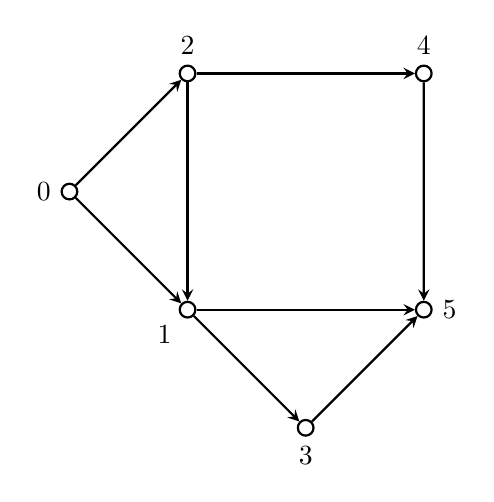
\begin{tikzpicture}
[nodedecorate/.style={shape=circle,inner sep=2pt,draw,thick},%
  arrowdecorate/.style={->,>=stealth,thick},scale=1.5]
%% nodes or vertices
\foreach \nodename/\direction/\navigate/\x/\y in {0/left/west/0/0,
  1/below left/south west/1/-1, 2/above/north/1/1, 3/below/south/2/-2,
  4/above/north/3/1, 5/right/east/3/-1}
{
  \node (\nodename) at (\x,\y) [nodedecorate] {};
  \node [\direction] at (\nodename.\navigate) {$\nodename$};
}
%% edges or lines
\path
\foreach \startnode/\endnode in {0/1, 0/2, 1/3, 1/5, 2/1, 2/4, 3/5, 4/5} {
  (\startnode) edge[arrowdecorate] node {} (\endnode)
};
\end{tikzpicture}
